%% Follow comments to support use.

%%%%%%%%%%%%%%%%%%%%%%%%%%%%%%%%%%%%%%%%%%%%%%%%%%%%%%%%%
%% STEP 1: Choose options for MSc / BSc / seminar layout and your bibliographic style
%%%%%%%%%%%%%%%%%%%%%%%%%%%%%%%%%%%%%%%%%%%%%%%%%%%%%%%%%

%%  Language: 
%%      finnish, swedish, or english
%%  Pagination (use twoside by default)  
%%      oneside or twoside,
%%  Study programme / kind of report
%%      csm  = Master's thesis in Computer Science Master's Programme;
%%      tkt = Bachelor's thesis in Computer Science Bachelor's Programme;
%%      seminar = seminar report
%%  For Master's thesis choose your line or track:
%%      (30 cr thesis, 2020 onwards, Master's Programme in Computer Science = csm)
%%      software-track-2020 = Software study track
%%      algorithms-track-2020 = Algorithms study track
%%      networking-track-2020 = Networking study track

\documentclass[english,twoside,censored,csm,software-track-2020]{HYthesisML} 


% If wanted, open new chapters only at right page.
% By default, "openany".
%\PassOptionsToClass{openright,twoside,a4paper}{report}
\PassOptionsToClass{openany,twoside,a4paper}{report}

\usepackage{csquotes}
%%%%%%%%%%%%%%%%%%%%%%%%%%%%%%%%%%%%%%%%%%%%%%%%%%%%%%%%%
%% REFERENCES
%% Some notes on bibliography usage and options:
%% natbib -> you can use, e.g., \citep{} or \parencite{} for (Einstein, 1905); with APA \cite -> Einstein, 1905 without ()
%% maxcitenames=2 -> only 2 author names in text citations, if more -> et al. is used
%% maxbibnames=99 as no great need to suppress the biliography list in a thesis
%% for more information see biblatex package documentation, e.g., from https://ctan.org/pkg/biblatex 

%% Reference style: select one 
%% for APA = Harvard style = authoryear -> (Einstein, 1905) use:
\usepackage[style=authoryear,bibstyle=authoryear,backend=biber,natbib=true,maxnames=99,maxcitenames=2,uniquelist=minyear,giveninits=true,uniquename=mininit]{biblatex}
%% for numeric = Vancouver style -> [1] use:
%\usepackage[style=numeric,bibstyle=numeric,backend=biber,natbib=true,maxbibnames=99,giveninits=true,uniquename=init]{biblatex}
%% for alpahbetic -> [Ein05] use:
%\usepackage[style=alphabetic,bibstyle=alphabetic,backend=biber,natbib=true,maxbibnames=99,giveninits=true,uniquename=init]{biblatex}
%

\addbibresource{bibliography.bib}
% in case you want the final delimiter between authors & -> (Einstein & Zweistein, 1905) 
% \renewcommand{\finalnamedelim}{ \& }
% List the authors in the Bibilipgraphy as Lastname F, Familyname G,
\DeclareNameAlias{sortname}{family-given}
% remove the punctuation between author names in Bibliography 
%\renewcommand{\revsdnamepunct}{ }


%% Block of definitions for fonts and packages for picture management.
%% In some systems, the figure packages may not be happy together.
%% Choose the ones you need.

%\usepackage[utf8]{inputenc} % For UTF8 support, in some systems. Use UTF8 when saving your file.

\usepackage{lmodern}         % Font package, again in some systems.
\usepackage{textcomp}        % Package for special symbols
\usepackage[pdftex]{color, graphicx} % For pdf output and jpg/png graphics
\usepackage{epsfig}
\usepackage{subfigure}
\usepackage[pdftex, plainpages=false]{hyperref} % For hyperlinks and pdf metadata
\usepackage{fancyhdr}        % For nicer page headers
\usepackage{tikz}            % For making vector graphics (hard to learn but powerful)
%\usepackage{wrapfig}        % For nice text-wrapping figures (use at own discretion)
\usepackage{amsmath, amssymb} % For better math

\singlespacing               %line spacing options; normally use single
\fussy
%\sloppy                      % sloppy and fussy commands can be used to avoid overlong text lines
% if you want to see which lines are too long or have too little stuff, comment out the following lines
% \overfullrule=1mm
% to see more info in the detailed log about under/overfull boxes...
% \showboxbreadth=50 
% \showboxdepth=50



%%%%%%%%%%%%%%%%%%%%%%%%%%%%%%%%%%%%%%%%%%%%%%%%%%%%%%%%%
%% STEP 2:
%%%%%%%%%%%%%%%%%%%%%%%%%%%%%%%%%%%%%%%%%%%%%%%%%%%%%%%%%
%% Set up personal information for the title page and the abstract form.
%% Replace parameters with your information.
\title{Public copyright licenses in Software Engineering: A Multivocal Literature Review}

\author{Akira Taguchi}
\date{\today}

% Set supervisors, use the titles according to the thesis language
% in English Prof. or Dr., or in Finnish toht. or tri or FT, TkT, Ph.D. or in Swedish... 
\supervisors{Prof. Tomi Männistö}

\keywords{open source, free / libre software, copyright, proprietary software, copyleft, license}
\additionalinformation{\translate{\track}}

%% For seminar reports:
%%\additionalinformation{Name of the seminar}

%% Provide classification terms, to appear on the abstract page.
%% Replace the classification terms below with the ones that match your work.
%% ACM Digital library provides a taxonomy and a tool for classification
%% in computer science. Use 1-3 paths, and use right arrows between the
%% about three levels in the path; each path requires a new line.

\classification{\protect{\\
Social and professional topics $\rightarrow$ Computing / technology policy $\rightarrow$ Intellectual property $\rightarrow$ Licensing \\
}}

%% If you want to quote someone special. You can comment this line out and there will be nothing on the document.
%\quoting{Bachelor's degrees make pretty good placemats if you get them laminated.}{Jeph Jacques}


%% OPTIONAL STEP: Set up properties and metadata for the pdf file that pdfLaTeX makes.
%% Your name, work title, and keywords are recommended.
\hypersetup{
    unicode=true,           % to show non-Latin characters in Acrobat’s bookmarks
    pdftoolbar=true,        % show Acrobat’s toolbar?
    pdfmenubar=true,        % show Acrobat’s menu?
    pdffitwindow=false,     % window fit to page when opened
    pdfstartview={FitH},    % fits the width of the page to the window
    pdftitle={},            % title
    pdfauthor={},           % author
    pdfsubject={},          % subject of the document
    pdfcreator={},          % creator of the document
    pdfproducer={pdfLaTeX}, % producer of the document
    pdfkeywords={something} {something else}, % list of keywords for
    pdfnewwindow=true,      % links in new window
    colorlinks=true,        % false: boxed links; true: colored links
    linkcolor=black,        % color of internal links
    citecolor=black,        % color of links to bibliography
    filecolor=magenta,      % color of file links
    urlcolor=cyan           % color of external links
}

%%-----------------------------------------------------------------------------------

\begin{document}

% Generate title page.
\maketitle

%%%%%%%%%%%%%%%%%%%%%%%%%%%%%%%%%%%%%%%%%%%%%%%%%%%%%%%%%
%% STEP 3:
%%%%%%%%%%%%%%%%%%%%%%%%%%%%%%%%%%%%%%%%%%%%%%%%%%%%%%%%%
%% Write your abstract in the separate file, to be positioned here.
%% You can make several abstract pages (if you want it in different languages),
%% in which case you should also define the language of the abstract,
%% as below.

% \begin{abstract}{finnish}

% Tämä dokumentti on tarkoitettu Helsingin yliopiston tietojenkäsittelytieteen osaston opin\-näyt\-teiden ja harjoitustöiden ulkoasun ohjeeksi ja mallipohjaksi. Ohje soveltuu kanditutkielmiin, ohjelmistotuotantoprojekteihin, seminaareihin ja maisterintutkielmiin. Tämän ohjeen lisäksi on seurattava niitä ohjeita, jotka opastavat valitsemaan kuhunkin osioon tieteellisesti kiinnostavaa, syvällisesti pohdittua sisältöä.


% Työn aihe luokitellaan  
% ACM Computing Classification System (CCS) mukaisesti, 
% ks.\ \url{https://dl.acm.org/ccs}. 
% Käytä muutamaa termipolkua (1--3), jotka alkavat juuritermistä ja joissa polun tarkentuvat luokat erotetaan toisistaan oikealle osoittavalla nuolella.

% \end{abstract}

\begin{otherlanguage}{english}
\begin{abstract}
	\textbf{Context:} Public licenses are central to the distribution of works in software engineering. For example in open source there must be an appropriate PCL attached to the source code in order for open-source software to be freely available for possible modification and redistribution. Understanding PCLs can be difficult. This could stem from the legal nature of the license texts and the large number of already-existing PCLs. As a result some actions made within the boundaries of the PCLs may come as a surprise to the public.
	
	\textbf{Objective:} The primary goal of this research is to conduct a multivocal literature review of the current state of PCLs in software engineering, the evaluation of the them and the evidence level of the research. The research aims to provide a novel perspective on relevant licenses and to extract key findings through a rigorous literature review process. This study has two main viewpoints: to provide rigorous research on PCLs to the academic field and to provide insights to the professional field of software engineering on PCLs. The grand goal of this thesis is to raise awareness of the importance of PCLs so that more licensers would make the correct choices based on their situations and needs in a mindful way.
	
	\textbf{Method:} The search strategy examined 6666 sources, found through websites that list PCLs and ad-hoc searches. Applying inclusion and exclusion criteria resulted in the selection of 666 sources, which made relevant contributions related to PCLs in software engineering.
	
	\textbf{Results:} 

	\textbf{Conclusions:} 
\end{abstract}
\end{otherlanguage}

\section*{Acknowledgements}
much love to suvi, artemis, sami nurmivaara, prof männistö and prof mäntylä

thanks to def for borrowing gpt4. thanks to rashid and barunes for sending me software licensing related videos and news. thanks to iikka and joonas for giving a hint for using a license database.

dedicated to suvi <3

% Place ToC
%\newpage
\mytableofcontents

\mainmatter

%%%%%%%%%%%%%%%%%%%%%%%%%%%%%%%%%%%%%%%%%%%%%%%%%%%%%%%%%
%% STEP 4: Write the thesis.
%%%%%%%%%%%%%%%%%%%%%%%%%%%%%%%%%%%%%%%%%%%%%%%%%%%%%%%%%
%% Your actual text starts here. You shouldn't mess with the code above the line except
%% to change the parameters. Removing the abstract and ToC commands will mess up stuff.
%%
%% Command \include{file} includes the file of name file.tex.
%% A new page will be created at every \include command, 
%% which makes it appropriate to use it for large entities such as book chapters. Cannot be nested.
%% It is useful for a big project, as changing one of the include targets 
%% won't force the regeneration of the outputs of all the rest.
%% Alternatively, \input is a more lower level macro 
%% which simply inputs the content of the given file like it was copy&pasted there manually.

\chapter{Introduction\label{intro}}
% setting
Public software licenses play a central role to the distribution of works in software engineering. For example in open source there must be an appropriate public software license attached to the source code in order for the piece of software to be freely available for possible modification and redistribution. Because open source is central to software engineering the licenses enabling open source must also be considered important in the same context.

% definition
Public license is defined by Wikipedia with the following words \citep{wikipedia:publiclicenses}:
\begin{quote}
	''A public license is a copyright license where the licensees are not limited. Examples include free content, open content, Creative Commons, free software and open source licences.''
\end{quote}

% problem
Understanding public software licenses can be difficult. This could stem from the legal nature of the license texts and the large number of already-existing public software licenses. The license texts usually favors correctedness over the readability for the developer. This is because the license text has to act as a valid legal instrument otherwise it cannot be endorsed \citep{ferguson2006gpl}. The lack of understanding of public software licenses leaves too much room for interpretation. In June 21, 2023 International Business Machines' (IBM) Red Hat seemingly violated the spirit of a popular public software license, the GNU General Public License version 2 (GPL-2.0) \citep{sfc:rhel} \citep{ibm:rhel}. This was an unpleasant surprise to the public. If the public software licenses would be more easily understood, the proprietarization of RHEL would have been less of a surprise to the users. To give some context on the violation of the spirit of the GPL-2.0, the project behind GNU General Public License (GPL), GNU Project initially attempted to ensure the users via the GPL have to the following three freedoms \citep{gnu:free}:
\begin{itemize}
	\item Freedom 1:	The freedom to study how the program works, and change it so it does your computing as you wish. Access to the source code is a precondition for this.
	\item Freedom2: The freedom to redistribute copies so you can help others
	\item Freedom 3:	The freedom to distribute copies of your modified versions to others. By doing this you can give the whole community a chance to benefit from your changes. Access to the source code is a precondition for this.
\end{itemize}

% easier sub-problem
On top of the legal details of public software licenses, software engineers in general have a tough time understanding the basic goals of public licenses used in software engineering. In the instance of the RHEL incident it would have been even lesser of a  surprise to software engineers if they would have known about other public software licenses and what they try to achieve, or how old is GPLv2 and why it has been succeeded by GNU General Public License version 3 (GPL-3.0).

% thesis contribution
This thesis' goal is to contribute into the solving these problems in a structured manner. First we state definitions and terminology used in the scope of this thesis. We go over the reasons why there does not exist consistent terminology in this area and conversely why the definitions are the most stabile ones in this area. Second we take a deep dive into the public software licenses through a multivocal literature review. To make more information available, a mapping study connected to the terminology scope defined in the first step is needed. Third includes our own suggestions and basic knowledge for professionals and academics in the industry to enhance the understanding of public licenses in software engineering. This step also includes discussion of the future research and contributes to stablizing the terminology and reinforcing the already-existing definitions in the academic field.

\section{Research goal, questions and contributions}
% primary object of this research (rqs)
The primary goal of this research is to conduct a multivocal literature review of the current state of public licenses in software engineering, the evaluation of the them and the evidence level of the research. The research aims to provide a novel perspective on relevant licenses and to extract key findings through a rigorous literature review process. The research questions of the review are:
\begin{itemize}
	\item RQ1: How many public software licenses are there in the top five software license listing cites?
	\item RQ2: How much is there disagreement in the shortcode names between different public software licenses listing sites?
	\item RQ3: How many public licenses in software engineering does there exist?
\end{itemize}

% 1.2 will examine terms
Terms such as open source, source code, free software and other vocabulary must be defined in the scope of this thesis. \hyperref[sec:bg]{Section 1.3} will examine this plethora of of terminology and definitions and will be used to establish a sound basis for discussing this broad subject.

% viewpoints
This study has two main viewpoints. The first one is to provide rigorous multivocal research on public software licenses to the academic field. Because this thesis already does the multivocal work on public licenses in software engineering, the researches of the future can cite the results of this thesis without having to mark their study a multivocal one. This is the grand goal of this thesis. The second one is to provide insights and general metrics to the professional field of software engineering on public software licenses. Hopefully this makes conversation on public licenses in software engineering easier and more rooted to scientific research rather than gut feeling and old, non-scientific articles on the insights and metrics of public licenses in software engineering.

\section{Thesis structure}
% thesis structure
This thesis follows the IMRaD structure. \hyperref[intro]{Chapter 1} introduces the problem, this thesis' possible contributions and some further background. \hyperref[methods]{Chapter 2} goes over the process and the methods of the multivocal literature review. This is where most of the actual research takes place in. \hyperref[results]{Chapter 3} presents results to the research questions. \hyperref[discussion]{Chapter 4} discusses implications for research. The chapter also discusses software engineering professionals in the thesis' context and the validity of the thesis' research. \hyperref[conclusions]{Chapter 5} concludes this thesis with the help of the research questions and the future of the research.

\section{Background and terminology of public licenses\label{sec:bg}}
% state of current terminology
The current terminology is used inconsistently which leads to incorrectness in the field of software engineering. For example The Open Source Initiative (OSI) classifies GPL-3.0 under the term ''open source'' whereas the Free Software Foundation (FSF) classifies GPL-3.0 under the term ''free software'' \citep{osi:gplv3}\citep{rms:opensource}. Some parts of the two definitions are mutually exclusive. This is rarely mentioned when people talk about Free and Open Source Software (FOSS) or Free / Libre and Open Source Software (FLOSS) which leads to misunderstanding that the two approaches are the same. This is why our focus will be public licenses in software engineering, and not for example, FLOSS licenses in software engineering. This also distinguishes our investigation from the broader topic of copyright licenses or the copyright law. This also includes public software licenses that are not approved by the FSF nor OSI hence not falling under the group of FLOSS licenses. In this section we aim to increase the accessibility of our discussion by providing a concise overview of the background of the field of public software licenses and the terms we employ.

% explain copyleft
Another example of term inconsistency is the term ''copyleft'',which is defined by \cite{mustonen2003} in the following way:
\begin{quote}
	''Copyleft is a novel licensing scheme. It facilitates open and decentralized software development. Its key feature is that once a program is licensed by the inventor, the subsequent programs based on the original must also be licensed similarly.''
\end{quote}
Like with the definition of sustainability \citep{weak-sustainability}, copyleft also has the definitions of weak and strong within the term \citep{wikipedia:copyleft}. Weak copyleft licenses are often used to cover software libraries. This allows other software to link to the library and be redistributed without the requirement for the linking software to also be licensed under the same terms. Strong copyleft shares the same features \cite{mustonen2003} presents regardless of the library nature of a piece of software. The general use of the term ''copyleft'' without the prefix also leads to inconsistency in the term usage.

% terms of other interest areas of the thesis
To explain our emphasis on public licenses in software engineering, it is essential to examine the other possible areas of interest in public licenses. Our study classifies such efforts into eight domains as mentioned by the GNU Project \citep{gnu:licenselist}. These domains include:
\begin{itemize}
	\item public licenses in software engineering
	\item public licenses in documentation for example architecture documentation of a project that may or may not be software or even publicly licensed
	\item public licenses in artistic works for example digital art, music or videos
	\item public licenses in educational works
	\item public licenses in fonts
	\item public licenses in viewpoints
	\item public licenses in physical objects
	\item public licenses in other works
\end{itemize}
The primary aim of this study is to investigate public licenses in software engineering process. However, it is important to acknowledge that public licenses in software engineering is only one aspect of public licenses in general. These additional dimensions are crucial in adoption and implementation of public licenses in software engineering, but they are not the focus of this thesis.

% acknowledge one example of non-focus
For example, including artistic works such as music would require us to understand the basics of music theory and what sets apart distinct pieces of music from one another, something that could be outside the skillset of the author. While developing a comprehensive theory, framework, and tooling for public licenses as a whole is a gargantuan task beyond the scope of a single thesis, narrowing our focus to software engineering enables us to examine a more concise and complete aspect of the main topic of this thesis.

% legal aspect scope
As significant point of clarification, it is essential to acknowledge that public licenses are generally meant to be used as valid legal instruments. The question whether or not a public license can act as a legal instrument is critical to the main function of these licenses. However, this thesis will not focus on the legal doctrine aspects either. The enforceability of public licenses has seen discussion in the academic field of law since the dawn of these licenses and since there's already an academic base for research it is likely the discussion seems to continue on with a healthy amount of activity \citep{duisburg2011gpl}.

% state of terminology standardization
Since the most recognized public licenses in software engineering are either open-source licenses or free software licenses and since both paradigms are driven by different organizations with different goals and values, it is understandable how non-standardized the terminology in the scope of public licenses in software engineering is. The example given in the first section of this sub-chapter illustrates the challenges involved in maintaining consistency in the use of terminology in this emerging field and further warrants a closer inspection of the terminology to emphasize our own standing in the field.

To provide an understanding of the terminology used in this thesis, a Venn diagram is presented in \hyperref[fig:terms]{Figure 1.1}, which contextualizes the non-standardized terminology within the PCL scope as a whole. This perspective provides an increased understanding of where different subdomains fall in the larger picture of PCLs. Furthermore it is essential to note that PCLs in software engineering encompasses different aspects that require a closer examination.

\begin{figure}[t]
	\centering
	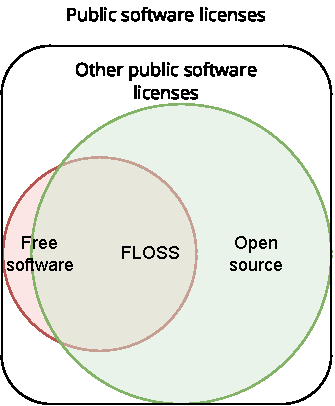
\includegraphics[scale=1.5]{figures/terms-diagram.pdf}
	\caption{PCLs in software engineering}
	\label{fig:terms}
\end{figure}

Let us explore further the differences and similarities between open source and free software at the software engineering level of PCLs. This is a crucial step since we can see from the approximation in \hyperref[fig:terms]{Figure 1.1} that the majority of PLCs are either free software, open source or both. We glanced over the free software definition in the first section of \hyperref[intro]{Chapter 1}. Open Source Initiative defines open-source licenses in the Open Source Definition briefly in the following way \citep{osi:licenselist}:
\begin{quote}
	''Open source licenses are licenses that comply with the Open Source Definition - in brief, they allow software to be freely used, modified, and shared.''
\end{quote}

Like the FSF with free software, OSI has the final word on what passes as open source and what does not. For example a new software PCL will not classify as free software nor open source until the corresponding organization has acknowledged the software PCL as either free software, open source or neither. If a PCL is accepted by both FSF and OSI it will fall under the term FLOSS. If a PCL gets accepted by neither of the organization or it gets rejected by both organizations it will fall under other software PCLs in the \hyperref[fig:terms]{Figure 1.1}. In general free software license requirements are considered more strict than the open source license requirements. For the sake of perspective we could simplify the differences like so: free software requires the redistributions of the licensed software to be open as well but open source does not require this. The terms free software and open source are in general often misunderstood or just thought of as FLOSS collectively because the terms have a hard time conveying their paradigms in the natural language. One would not think free software does not mean software free of charge nor would one think that open source allows closed source redistributions of the licensed software. We will glance over the impacts on the industry of these two terms in \hyperref[discussion]{Chapter 4}.

With the context laid out in this chapter let us define PCLs in software engineering for the purpose of this study: Public software licenses are copyright licenses where the licensees are not limited and the copyright license in question is meant be used in licensing software source code. This helps us create the search strings and find the relevant literature for this thesis. This also helps us exclude PCLs regarding documentation, media and all other non-software targeted PCLs.

% acknowledge the topic is complex
The quest to categorize every software PCL under some paradigm objectively is a complex one and cannot be comprehensively answered in a single paragraph. Therefore it is essential to continue taking the correct steps towards incresing the scientific understanding and providing the industry with examples, standards and processes to follow. However, as the following chapters reveal, a significant amount of effort is still being spent on solving the same problem multiple times, rather than building on existing knowledge and finding the next problem to solve. This thesis aims to contribute to mitigating this challenge by providing a rigorous analysis of the current state of the field. As the knowledge, conventions, and terminology take shape,we can look forward to reaching a state where less effort is spent on defining concepts and more on practical problem-solving.
\chapter{Methods\label{methods}}
% aim of the chapter
This chapter aims to establish a precisely defined and rigorous research approach to enhance transparency and repeatability. We will take the steps required to ensure that every phase and decision is thoroughly documented, enabling the reader to retrace the research process. In a thesis made by a single researcher, the lack of cross-examination of results with multiple researchers and the validation of evaluation criteria for opinion bias pose threats to validity, as will be clarified further in \hyperref[discussion]{Chapter 4}. Therefore, special attention will be paid to address these concerns. By following this approach, this research endeavors to contribute to the existing body of knowledge in the field of computer science in a robust and reliable manner.

\section{Overview of the process}
% explain slr
The systematic literature review method is a well-established approach for conducting a comprehensive and rigorous analysis of the existing research on specific research question or subject \citep{kitchenham2007}. This paper presents a multivocal literature review. Multivocal literature review is type of systematic literature review that includes both academic literature and grey literature \citep{mantyla2019}. This method was selected for this study to facilitate a thorough and scientifically interdisciplinary examination of public licenses in software engineering. The existing literature consists of public software licenses not found in academic databases and as such are considered gray literature, making the thesis a multivocal literature review.

% kitchenhamn 2007
This study follows the guidelines outlined by \cite{kitchenham2007}, to ensure its quality. The multivocal review method consists of three distinct phases: planning, conducting and reporting the review. This study stricly adhered to this structure. The phases can be further broken down into a research protocol, as illustrated in \hyperref[fig:slrphases]{Figure 2.1}. Adhering to the protocol is the first step in ensuring a well-documented and rigorous process, which increases the validity and auditability of the study.

\begin{figure}
	\centering
	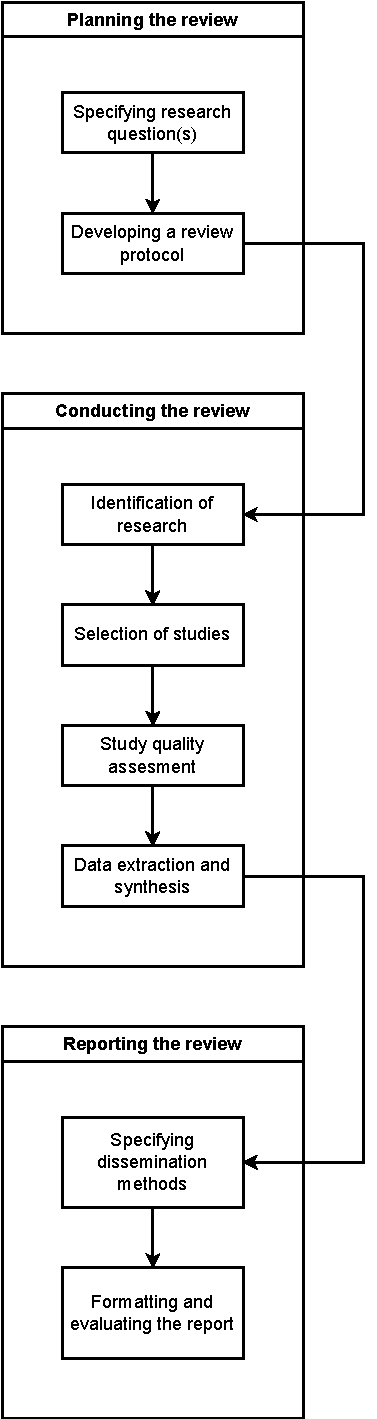
\includegraphics[scale=0.9]{figures/slr-phases.pdf}
	\caption{Three phases of a systematic literature review}
	\label{fig:slrphases}
\end{figure}

% how our slr came to be
The multivocal literature review process began with the formulation of research questions and the establishment of a comprehensive search strategy and scope. The search process was conducted by employing a quasi-gold standard (QGS) approach based on the implementation by \cite{qgs}. After the completion of the search process, the inclusion and exclusion criteria were defined. To ensure a structured evaluation of the literature, a data extraction form was created. Finally, a strategy for analyzing the extracted data from the literature was designed.

% reliability and validity
 To ensure the reliability and validity of the research protocol, it was validated against similar systematic literature reviews in computer science, the aforementioned guidelines by \cite{kitchenham2007}, and was further refined through an iterative process. Specifically, a subset of the data was tested on (The QGS) and any identified issues or problems were recorded and addressed. The details of this process are explained and thoroughly documented in the following sections. Similarly, the same approach was followed for the data extraction process, whereby a subset of literature was tested to refine the data extraction form. The revision of the form was undertaken as necessary to guarantee the completeness and accuracy of the extracted data.

 \section{Research questions}\label{rqs}
 % purpose of rqs
The research questions in this study served two primary purposes. Firstly, they aimed to provide an analysis of the existing multivocal literature on public licenses in software engineering for the researchers interested about the field. Secondly, the questions were designed to cater a secondary audience of professional software engineering practicioners. As discussed in the \hyperref[intro]{Chapter 1}, the following research questions were addressed in this thesis:

\begin{itemize}
  \item RQ1: How many public licenses in software engineering does there exist?
  \item RQ2: How consistent are the naming conventions for public licenses in software engineering
\end{itemize}

% aim of rq1
The multivocal literature review in this thesis begins with addressing RQ1, which aims to provide the amount of public software licenses that exist in our five public license listing sites in total. This information could be valuable for researchers but mostly it could be valuable to the practitioners since it could give some overview and a sense of the scale when picking a public software license that would serve the practitioners' needs the best. The results can be used to introduce some notable background of the current public licenses in software engineering and enabling focus to more specific areas inside the topic of this thesis.

Next RQ2 seeks to find the amount of duplicate licenses between the license listing sites. Results to this research question are also mostly useful to researchers of the field. The results give an overview of the naming consistency for these public software lienses. Moreover, the documented methods are most likely the most valuable information for the researchers.

Finally RQ3 attempts to count the total number of individual public software licenses within the scope of this thesis. The research question builds on top of the results and methods of the previous research questions. This information could be most valuable for the practitioners 

\section{Search strategy}
% where was search process conducted in (inclusion/exclusion in appendix a)
The search process was conducted on five public license listing websites. The selection criteria for the literature were defined after the search process and the selection process was based on inclusion and exclusion criteria. The inclusion and exclusion criteria and each step of exclusion on the literature found are presented later in this chapter. Originally the search terms would have been applied to the license listing sites directly just like in a normal multivocal literature review or in a systematic literature review. Keywords however produced highly varying and non-reproducible results in Google Scholar and Google Search. Some license listing websites such as FSF's list of pages categorized as licenses could not be found from Google Search even with the \texttt{site} operator: \\
\texttt{site:https://directory.fsf.org/wiki/Category:License}. Although the page has been up since 2013, for some reason Google has not crawled the page in 10 years \citep{fsf:licenselist}. This is why this thesis does not include search terms of the initial phase per se but rather inclusion and exclusion strings on the second phase. For the sake of validity the thesis still follows the guidelines presented in \cite{kitchenham2007} with the exception of replacing an academic database search engine with the five license listing sites, web scraping and our own Python script performing the legwork of an academic database search engine in a systematic literature review.

% data extraction process
The data extraction process was performed in a standardized and systematic manner, with the aim of obtaining the relevant information from the selected literature. The data extraction form used included license shortcode used in the listing site, listing site name, full license text and is available  \hyperref[table:listing-sites]{Table 2.1}. The extracted data was then used to answer the research questions and perform the data analysis. The results of the data analysis were then reported in a rigorous manner.

\begin{table}[t]
  \caption{License listing sites chosen}
	\begin{center}
		\begin{tabular}{||l l||}
			\hline
			URL & Shortcode \\
			\hline
      https://spdx.org/licenses/ & SPDX \\
      https://wiki.debian.org/DFSGLicenses & DFSG \\
      https://directory.fsf.org/wiki?title=Category:License & FSF \\
      https://opensource.org/licenses & OSI \\
      https://www.gnu.org/licenses/license-list.html & GNU \\
			\hline
		\end{tabular}
		\label{table:listing-sites}
	\end{center}
\end{table}

% more on where was search process conducted in
\subsection{Search method}
The search was conducted on five license listing websites shown \hyperref[table:listing-sites]{Table 2.1}, as mentioned earlier, to obtain a broad set of multivocal literature. This approach yielded a large number of literature that were processed to a subset of high-relevance literature using inclusion and exclusion criteria presented later in this chapter. Manual searching of databases with hundreds of public licenses is not feasible, and it is prone to researcher bias and may overlook relevant venues from other scientific disciplines. However, a preliminary manual search was performed to reduce the number of iterations required and establish the quasi-gold standard (QGS) mentioned earlier.

% how were search terms determined
\subsection{Search scope and terms}
The search terms, or in our case, the inclusion and exclusion string was determined through an iterative process that took into account the research questions and topic. Synonyms for key terms were included and combined using Boolean logic to form a comprehensive inclusion and exclusion string. As mentioned earlier the inclusion and exclusion criteria are presented later in this chapter.

% qgs on search string
The inclusion and exclusion string was established on a basis of quasi-gold standard as proposed by \cite{qgs}. For establishing a quasi-gold standard we employed a manually crafted inclusion and exclusion string based on the topic and research questions of this study. As we defined public licenses in software engineering as licenses where the licensees are not limited and the license in question is meant be used in licensing software source code in \hyperref[intro]{Chapter 1} and our research questions focus on finding useful metrics about the public licenses, we manually formulated the inclusion and exclusion string in Python:
\begin{verbatim}
  ^(?!.*\b(documentation\s+license|creative\s+commons|open data)\b).*
\end{verbatim}
% web scrape beginning
In order to run the inclusion and exclusion string that established the quality-gold standard against the literature we had to gather them first. We started defining our search scope from the Wikipedia page of one of the most used open source license \citep{github:licenseusage}, the MIT license \citep{wikipedia:mit}. The infobox contained fields in the order shown in \hyperref[table:infobox]{Table 2.2}.

\begin{table}[t]
  \caption{MIT License Wikipedia page infobox}
	\begin{center}
		\begin{tabular}{||c c||}
			\hline
			Field & Value \\
			\hline
			Publisher & Massachusetts Insitute of Technology \\
			SPDX identifier & MIT \\
			Debian FSG compatible & Yes \\
			FSF approved & Yes \\
			OSI approved & 	Yes \\
			GPL compatible & Yes \\
			Copyleft & No \\
			Linking from code with a different license & Yes \\
			\hline
		\end{tabular}
		\label{table:infobox}
	\end{center}
\end{table}
The validity threats regarding this choice are discussed in a later chapter. The publisher, GPL compatibility, copyleft and the linking exception did not result in any meaningful license listing websites. This leaves us with the SPDX, Debian FSG compatibility, FSF and OSI from which all resulted in some sort of license listing websites. Since the fields were roughly as follows: SPDX, FSF, OSI and GNU, after some investigating, we decided to start the search for public software licenses from the following license listing sites:

% how many results
The web pages were scraped of the public license shortcodes using the browser's developer tools. These shortcodes were imported into a spreadsheet editor with each shortcode under their corresponding listing site name. This resulted in over 1000 public licenses. Because the same public license would sometimes occur in multiple listing sites strictly duplicate shortcodes were removed using the spreadsheet editor resulting in 780 public licenses. Removing the duplicates was not intelligent and left duplicates like ZPL-2.0 and ZPL - 2.0 as unique license shortcodes. The solution to this problem is presented in a later sub-chapter. The table in the state after the strict removal of duplicates is provided in this thesis' repository \footnote{\url{https://github.com/akirataguchi115/mscthesis/}} under the name of \texttt{stage1-licenses.md}.

With the search for the initial license listing websites completed we moved onto the search process itself.

\section{Search process}
% Study selection divided into multiple stages (figure)
The literature selection process was divided into multiple stages, as outlined in \hyperref[fig:search-process]{Figure 2.2}. The initial step involved the formation of a inclusion and exclusion string through the use of a quasi-gold standard.

\begin{figure}
	\centering
	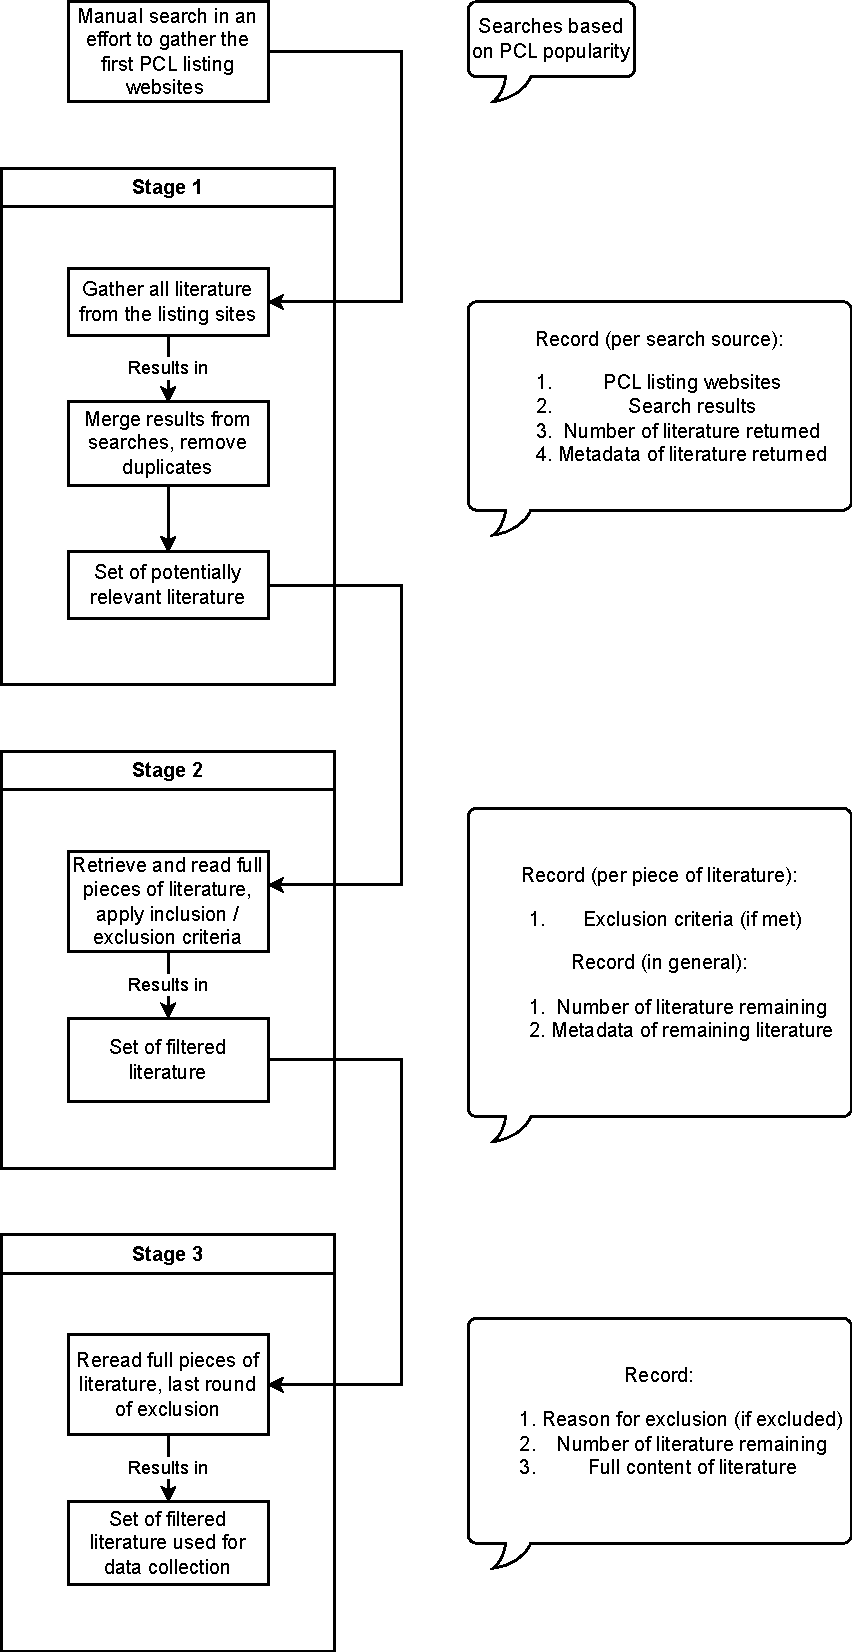
\includegraphics[scale=0.67]{figures/search-process.pdf}
	\caption{Search process divided into stages}
	\label{fig:search-process}
\end{figure}

% first stage
In the first stage, the search was conducted using the web pages titled  ''MIT License'' \citep{wikipedia:mit}, ''SPDX License List'' \citep{spdx:licenses}, ''The DFSG and Software Licenses'' \citep{debian:dfsg}, FSF's ''Category:License'' Wiki page \citep{fsf:licenselist}, GNU's ''Various Licenses and Comments about Them'' \citep{gnu:licenselist} and "OSI Approved licenses" \citep{osi:licenselist} focusing, focusing on the license listing site name and shortcode. Then we identified and eliminated any duplicates, producing a preliminary set of potentially relevant literature. The dataset after the first stage of the search process is provided in this thesis' repository \footnote{\url{https://github.com/akirataguchi115/mscthesis/}} under the name of \texttt{stage1-licenses.md}., as mentioned earlier.

%second stage
In the second stage, the inclusion and exclusion criteria were applied to further filter the literature and reduce the number of licenses to be reviewed. Then the resulting dataset was taken for a closer look where the quality of the literature was examined manually by the author, resulting in some manual exclusions based on the content and availability of the literature. This is where the inclusion and exclusion string took concrete place in which means the results were cross-referenced with the quasi-gold standard to validate it. The verbal reasoning for manual exclusions is clarified in \hyperref[incexc-criteria]{Sub-chapter 2.4}. The dataset after the second stage is provided in this thesis' repository \footnote{\url{https://github.com/akirataguchi115/mscthesis/}} under the name of \texttt{stage2-licenses.md}.

% third stage
The third stage was the most time-consuming and involved a manual review of the full license texts. After reading and evaluating each license, a final round of exclusions was completed and documented. The remaining licenses were used for data collection and analysis in the final part of the study. The final list of licenses is available in \hyperref[appendix:a]{Appendix A}.

% fetch licenses from scancode
\section{Inclusion and exclusion criteria\label{incexc-criteria}}
Before we could apply the inclusion and exclusion criteria to the literature we had to fetch the full license texts from somewhere since the first stage's dataset included only the shortcode and listing site name. We decided that the public license database by ScanCode published in GitHub \citep{scancode} was to be used fetching the initial full license texts based on the shortcodes of the first stage. The license database could be found by searching GitHub with the term ''license database''. The monolithic Python script used for this matching and fetching is provided in this thesis' repository \footnote{\url{https://github.com/akirataguchi115/mscthesis/}} under the name of \texttt{methods.py}. Some shortcodes from the first stage did not match any full license texts from the license database. We had to manually fetch the missing full license texts from these license listing sites. The fetching was done systematically in cycles until no more missing full license texts were found with the help of the first stage spreadsheet. as can be seen from the Python script. We now had a complete Python dictionary with the shortcode as the key and full license text as the value.

% incl excl regex string
To be eligible for the data collection and analysis, a license had to match the following inclusion and exclusion regular expression string:
\begin{verbatim}
  ^(?!.*\b(documentation\s+license|creative\s+commons|open data)\b).*
\end{verbatim}

% comments on applying
The regular expression string first included some inclusion matching but we soon realized it would be more efficient to exclude licenses than to include licenses. To establish the quasi-gold standard we first tried to exclude all full license texts including the words ''creative commons'' since we knew the Creative Commons licenses are not suitable for computer code, which is our scope. We then opened all excluded licenses into tabs in our text editor which the Python script assigned to their respective directory of excluded licenses based on the regular expression. We then looked quickly at the first few lines of the full license texts and judged if the license was indeed not suitable for our scope. Then we did the same to the included licenses in their respective directory and glanced if there were some types of licenses that were not suitable for our scope. We did one more cycle like this to finally exclude the string ''documentation license'' as well. During the two cycles we manually marked some licenses as included or excluded regardless of the regular expression matching since there did exist some corner cases the matching missed. This ended the second stage of search process which focused on inclusion and exclusion criteria.

% what was done to answer rq (table data extraction form)
\section{Data collection and data analysis}
To answer the research questions of this thesis, a thorough examination of the selected primary literature was conducted and the necessary data was collected using data extraction form presented in \hyperref[table:extraction]{Table 2.3}. A record of the full license texts after the third stage was kept for anaysis and is available as a directory called \texttt{stage3-licenses} in the thesis' repository \citep{mscthesis}.

\begin{table}[t]
  \caption{Data extraction form}
	\begin{center}
		\begin{tabular}{||c c c||} 
			\hline
			\# & Field & Concern/Research question \\
			\hline
			F1 & Shortcode & RQ2, RQ3 \\
			F2 & Listing site name & RQ1, RQ2 \\
			F3 & Full text &  Documentation\\
			\hline
		\end{tabular}
		\label{table:extraction}
	\end{center}
\end{table}

% third stage how to
To get the necessary from the remaining literature we decided that the next reasonable step was to remove duplicates from the licenses as systematically as possible. We used Python's \texttt{difflib} library to sort the full license texts. The library itself used the Ratcliff and Obershelp algorithm compare every full license text to every full license text. The time complexity is $O(n^3)$ and $\theta(n^2)$. This took our working computer 68 minutes each time the algorithm ran so we decided to only do one cycle of this type of duplicate removal. The licenses were outputted to \texttt{duplicate-finding} directory with the naming convention of \texttt{n-shortcode.txt} where the n was the sort order given by the Ratcliff and Obershelp algorithm. We then opened these licenses to tabs in our text editor and compared the full license texts by human eyes if they were actually the same license with little to no noise difference in the full license texts. The comparison tool of our text editor was also a helpful automation tool for longer licenses that could not fit into one computer display as whole without scrolling. ''open data'' was also applied in the regular expression string at this stage. While this should have happened in stage 2, we wanted to be honest that this exclusion really did happen in stage 3. At this stage we also manually excluded individual licenses from the final dataset if there was too much noise. For example, GNU listed licenses often as whitespaces or something alike.  Examples of these will be given in \hyperref[results]{Chapter 3}. This ended the third stage of the search process and provided us with the necessary data to answer the research questions.

%  next chapter presents outcomes
The subsequent chapter presents the outcomes of the steps taken in the study, as discussed above.
\chapter{Results\label{results}}

\chapter{Discussion\label{discussion}}
% indications
This research indicates that the field of public licenses in software engineering, meaning public software licenses, is at an early stage of development. The review of existing literature reveals a notable absence of common set of definitions and terminology in this field. Consequently, this often leads to work covering the same ground. Furthermore, the variability of terminology across different literature makes it challenging to compare and synthesize results effectively. Addressing this challenge will require the development of common measurement tools and frameworks for evaluating and comparing public licenses in software engineering. Such efforts could lead to the establishment of widely adopted standards for measuring and improving public software licenses.

% follow-up observation
That said, there is clear interest in public licenses in software engineering. Although the amount of purely academic literature on public software licenses is limited, the amount of grey literature on public software licenses is ever increasing. This is most likely due to the recent developments in the field regarding proprietarization noted in the \hyperref[intro]{Chapter 1}. 

% notable observation
A notable observation of our reserach is that the recent efforts in the industry have led to the development of Post Open Source not yet noted in the research literature reviewed \citep{register:poss}. Whether or not this paradigm will change the industry like open source and free software did will only be evident over time. The paradigm is explained shortly in \hyperref[conclusions]{Chapter 5}.

% acknowledge the topic is complex
The quest to objectively categorize every public software license is a complex one. Therefore it is essential to continue taking the correct steps towards incresing the scientific understanding and providing the industry with examples, standards and processes to follow. However, as the previous chapters have revealed, a significant amount of effort is still being spent on solving the same problem multiple times, rather than building on existing knowledge and finding the next problem to solve. As the knowledge, conventions, and terminology take shape,we can look forward to reaching a state where less effort is spent on defining concepts and more on practical problem-solving.

\section{Implications for research}
% how to generally improve scientific scene 1
To improve the maturity of research methods employed in the field of public licenses in software engineering, researchers should aim to use more rigorous and comprehensive research methods. This may involve using larger and more diverse data sets, developing more sophisticated measurement tools, and conducting experiments that are representative of real-world scenarios.

% how to generally improve scientific scene 2
Furthermore, researchers should strive to increase the transparency and reproducibility of their research by making their data and code openly available. This would enable other researchers to replicate and build upon their work, as well as facilitate the establishment of common standards and best practices.

% improve scientific scene multivocal vs academic
Finally, it is important for researchers to publish more articles regardless of the grey literature included in the papers. Because there is largely only grey literature published in the twenty-first century in the field, the next academic articles will be multivocal by default. The non-multivocal, academic articles will follow but only after there are systematic, academic and multivocal articles published for the former to build on. The results presented here are modest but by working together, researchers and industry professionals could produce more useful research regarding public licenses in software engineering.

\section{Implications for software engineering professionals}
% how to improve professional scene 1
Software engineering professionals should start by educating themselves of the basics of public licenses in software engineering and incorporating it into their design and development processes. They should be mindful or strive to mindful about the public licenses their third-party softwares are using and how it impacts their craft. Making a map of the public software licenses and their corresponding usecases might help plotting the larger picture.

% how to improve professional scene 2
However, it is important to acknowledge that the institutions should hold the greater responsibility of teaching the basics of public software licenses without getting too tangled up in history, politics or simply waving the field of as a form of human rights activism. The key focus points here being vocational schools, software engineering courses, college and university since these are the timestamps where most software engineers start to produce code that need to be licensed or require the use of a licensed piece of software.

% overall implications
Overall, the lack of public software license knowledge regarding software engineering professionals points to the need of more education regarding public software licenses and the practical effects stemming from the application of these licenses.

\section{Limitations and threats to validity}
The major limitation of this study is that the subjective results could not be validated by multiple researchers. In a systematic review, it is standard practice and highly recommended to have at least two, if not more, individuals independently conduct the review processes and then cross validating the findings. This would result in the possibility of comparing individual exclusion decisions and other decicions, thereby increasing the credibility of the study. However, in this study, the methodology was thoroughly documented, which allows us to assert with confidence that the study has an appropriate level of of validity.

As a work of single researcher, there is also a chance of inaccuracy and bias in the literature selection and filtering process. As much of the literature had to be reviewed manually and then included/excluded on a qualitative basis, this is a known limitation and a threat to validity. Multiple rounds of documented filtering and a clear paper trail of all decisions made keeps this threat in the acceptable levels.

\subsection{Limitations of literature selection for review}
Efforts were made to ensure the inclusion of comprehensive set of literature in the search process. This was achieved by setting the starting point of license listing sites to the Wikipedia article of the MIT license.

The first phase of filtering has some notable limitations starting with the two license listing websites: SPDX and DFSG. Since the material was gathered to a spreadsheet program the duplicates were removed using the short identifier the listing page was using. Let's look at this validity threat using an example. Suppose our spreadsheet program has acquired the public license with an identifier ''MIT''. The results of phase one will not include any other public license marked with the identifier ''MIT''. In the worst case the identifier ''MIT'' could have actually been ''MIT-DFSG-edition'' but with the identifier of ''MIT''. Since there were so many public software licenses in phase one it would not have been possible to check the uniqueness of all removed duplicates. One of the reasons why this would not have been feasible is that the listing sites would fetch the public license contents from another webpage or at the second worst case, from another website. The worst case is that the URl is dead and we get HTTP 404. The amount of public software licenses, duplicates and the lack of already existing tools makes this problem multilayered. However this is the level of integrity we decided to finish our study with.

FSF's license listing introduced us to pick another limitation for the scope of this thesis. The license shortcoded as ''other'' was not a public license but instead a hyperlink to another listing webpage that listed programs that the FSF has no yet managed to document the license which the program uses. Although the one of the programs called ''babl'' was licensed as with ''gplv3'' the amount of undocumented programs was over 5200 at the time of observation. For this reason we are excluding the public software licenses found indirectly from the category ''other''.

GNU project's listing site allowed us to use a shortcut of sorts which we will document here for the purposes of acknowleding the limitations of it. The table of contents at the listing site marked certain consequtive public software licenses as software public software licenses. On top of this the public software licenses were not organized into easily processable tables but rather in stacked on one another in rich text format. Although we decided to use regex on the HTML file the included public software licenses were only the ones that were simply under the header ''Software licenses''. In the worst case scenario GNU project could have misinterpreted some public software licenses as non-software licenses thus making this thesis exclude them with a wrong reason. While from a quick glance and the existence of the other four license listing sites, we think it is still worth documenting when it comes to validity and the integrity of this thesis.

On top of too heavy filters we would also like to document the too light filters in the literature selection for review. We can see from \hyperref[appendix:a]{Appendix A} that for example public software licenses with the literature identifiers L777 and L780 are almost the same regarding the shortcoded identifiers: ''ZPL - 2.1'' and ''ZPL-2.1''. The duplicate removal would have been seemingly simple to execute on phase 1. However with the presence of over 700 pieces of literature we decided not to give special treatment to any potential set of duplicates. While it is most possible that OSI's ''ZPL - 2.1'' is equivalent exactly to SPDX's ''ZPL-2.1'' we could not be sure without looking at their contents. This could have resulted duplicate public software licenses in the literature selection for review but these type of duplicates are removed in phases 2 and 3 due to the public software licenses being read in full.

% Miscellaneous validity issues on literature selection 
To finish this subsection we will discuss some more minor validity issues that did not fit into \hyperref[results]{Chapter 3} but are regardless important to note for the integrity of the thesis. Stage three of the search process included a validity threat regarding the removal of duplicates. If two full license texts would seem duplicates we would check the two license listing sites' license pages for further investigation without using an internet archiver. This is a common validity threat on this thesis, that is not relying on an internet archiver on every source possible. Still, archiving more than a thousand license pages and accessing them would have been very slow process in terms of both archiving and accessing.

% why exclusion over inclusion
As can be seen in  \hyperref[methods]{Chapter 2} the regular expression string was only an exclusion filter. Using an inclusion and exclusion resulted in difficulities to match all of the public software licenses. In other words it eventually turned out to be faster to match the excludable licenses than the includable licenses. The validity threat lying here is that only using an exclusion filter implicates a majority of the public licenses in our dataset to be public software licenses. An example of difficult to include public software license is the \texttt{wtfpl} which includes no evidence of it being a public software license but rather a general public license. However because \texttt{wtfpl} is a largely used in software source code as can be seen in \hyperref[results]{Chapter 3}. Another examples to back up this choice in exclusion-only are the font licenses that are considered public software licenses. With the exceptions inflating the inclusion regular expression string we eventually decided to only use the aforementioned exclusion filter. Before the decision our inclusion string looked like this:
\begin{verbatim}
  (.*\b(source|software|program|code|module|public(s+)license|ware|
  (w+)ware)\b).*
\end{verbatim}

As mentioned earlier in the thesis the Wikipedia infobox order of license listing sites plays a heavy role in the literature selection. This manifests as a validity threat for example in removal of duplicates where the duplicates are removed from the lattermost listing site, giving a false sense of the majority of the public licenses coming from the formermost license listing sites like the SPDX. While this might be true due to the high volume of literature from the formermost license listing sites in order of the Wikipedia infobox it is still a threat to validity. Because of this choice in our scope the accuracy of the origins of the licenses in the search stages is not as high as it could be.

FSF license listing site also had some other more minor issues than described earlier. Licenses like \texttt{DejaVu} and \texttt{DBG-3.0} did have an FSF license page found from the listing site but these pages only offered one single whitespace character as the full license text. Licenses like \texttt{CorkForkPL} also contained a whitespace as the full license text but included a note about a software that uses this license. Sometimes the full license text could be found by just clicking the provided hyperlink to the software mentioned which is what we did with \texttt{JahiaCSL}. Sometimes it would have required the author to download and unarchive source code to see the full license text or use an internet archiver on top of that due to broken hyperlinks or the software's website being down permanently. We solved this dilemma by deciding to only get the full license text if it was at maximum one click away from the original license listing page. In cases where the license was listed on the FSF license listing page as whitespace the full license text was fetched from the next license listing site in the Wikipedia infobox order if it existed there. For example the full license text for FSF's \texttt{MPL} was fetched from GNU under \texttt{MPL-1.1}. While we figured out reproducable rules to our literature selection phase it is fair to note that these are threats to validity regardless of the systematic nature of the remedies presented here.

A more general note on the systematicity of this thesis is due. Systematic does not equal to automatic. The author's human eyesight was for example a major factor to distinguish duplicates in literature selection in search stage three. Licenses were sorted by the Ratcliff and Obershelp, opened all search stage two licenses to tabs on the text editor, switched with keybinds between $n - 1$, $n$ and $n + 1$ full license texts and removed licenses that the author concluded to be duplicates based on various factors descrbied in \hyperref[methods]{Chapter 2}. As can be seen the process is systematic and relies heavily on the use of various automated tools but much of the work is also on the responsibility of the author's eyesight, memory and overall judgement which makes this process far from automatic. It is also good to note that the Python script used in \hyperref[methods]{Chapter 2} does not work on Windows systems. This was tested to decrease the waiting time of the Ratcliff and Obershelp on a more powerful desktop computer. This is the last and most minor validity threat mentioned in this thesis regarding the literature selection for review.

As mentioned in the beginning of this section, efforts were made to ensure the inclusion of comprehensive set of literature in the search process. However, as with all systematic literature reviews, a comprehensive manual review of all literature would have been a formidable task. Therefore, additional filtering was conducted. This filtering was carried out in two phases, starting with the application of inclusion/exclusion criteria, followed by a second phase focused on evaluating the nature of the public software licenses and conducting a manual review. As a result of this second phase, a set of literature were excluded following a critical appraisal, with documentation and reasoning provided for each section.

As such we can note that the literature selection was done in a sufficient manner.

\subsection{Limitations in data extraction}
% importance of data extraction
The process of data extraction holds great significance in a systematic literature review, as it has a direct impact on the transparency and rationale of the paper. The data extraction approach was shallow due to the data extraction form being relatively small. As mentioned above, not much data could be easily nor verifyiably extracted from our main grey literature, the five license listing sites. Despite the dilligent efforts to eliminate researcher bias, which is a common concern in interpretive methods, it was not feasible to replicate this work by another individual for cross-referencing purposes. However, the study's validity can still be considered appropriate, due to the transparent steps taken and the use of a short, but well-defined data extraction format.

% lack of measurements and tooling
We still note that because of the lack of common standardized measurements and tooling for them, a considerable amount of personal consideration had to be done to bring the research results of the primary literature into a comparative state.
\chapter{Conclusions\label{conclusions}}
\textcolor{red}{primary objective of this study}

\textcolor{red}{conclusions from each rq}


\section{Future research}
\textcolor{red}{adopting a clear baseline}

\textcolor{red}{why agplv3re is the best license}

\textcolor{red}{Docker CLA, SSPL}

\textcolor{red}{make cla easier maybe with gpg / joplin easy cla sign}

\textcolor{red}{LICENSE highlighting.js}

\textcolor{red}{what kind of efforts and why}

\textcolor{red}{what this thesis has provided}

%%%%%%%%%%%%%%%%%%%%%%%%%%%%%%%%%%%%%%%%%%%%%%%%%%%%%%%%%
%\cleardoublepage                          %fixes the position of bibliography in bookmarks
%\phantomsection
\addcontentsline{toc}{chapter}{\bibname}  % This lines adds the bibliography to the ToC
\printbibliography

%%%%%%%%%%%%%%%%%%%%%%%%%%%%%%%%%%%%%%%%%%%%%%%%%%%%%%%%%
\backmatter
\begin{appendices}

\appendix{Primary literature identified in the search process and their inclusion/exclusion
criteria\label{appendix:a}}

\begin{table}[h]
	\begin{center}
		\begin{tabular}{c | c | c} 
			\hline
			Literature identifier & Name & Year\\
			\hline
			S1 & MIT License & 1987 \\
			S2 & Apache 2.0 & 666 \\
		\end{tabular}
		\caption{A list of literature and the basic filtering step.}
		\label{table:appendix:a}
	\end{center}
\end{table}
\appendix{Primary literature reviewed, read in full and inclusion/exclusion criteria applied\label{appendix:b}}

\begin{longtable}[h]{m{2cm} | m{7cm} | c | c | c | c | c}
  \caption{List of literature with the inclusion/exclusion criteria applied.} \label{table:appendix:b} \\
  \hline
  Literature identifier & Identifier & SPDX & DFSG & FSF & OSI & GNU \\
  L1 & 0BSD & SPDX &  &  & OSI &  \\
  L2 & 996 &  &  & FSF &  &  \\
  L3 & AAL & SPDX &  &  & OSI &  \\
  L4 & Abstyles & SPDX &  &  &  &  \\
  L5 & AcademicFreeLicense &  &  &  &  & GNU \\
  L6 & ACDL-1.0 &  &  & FSF &  &  \\
  L7 & ACEL &  &  & FSF &  &  \\
  L8 & AdaCore-doc & SPDX &  &  &  &  \\
  L9 & Adobe-2006 & SPDX &  &  &  &  \\
  L10 & Adobe-Display-PostScript & SPDX &  &  &  &  \\
  L11 & Adobe-Glyph & SPDX &  &  &  &  \\
\end{longtable}
\appendix{Primary literature reviewed, read in full and data extracted\label{appendix:c}}

\begin{longtable}[h]{m{2cm} | m{7cm} | c | c | c | c | c}
  \caption{Final list of literature and their data extraction.} \label{table:appendix:c} \\
  \hline
  Literature identifier & Identifier & SPDX & DFSG & FSF & OSI & GNU \\
  L1 & 0BSD & SPDX &  &  & OSI &  \\
  L2 & 996 &  &  & FSF &  &  \\
  L3 & AAL & SPDX &  &  & OSI &  \\
  L4 & Abstyles & SPDX &  &  &  &  \\
  L5 & AcademicFreeLicense &  &  &  &  & GNU \\
  L6 & ACDL-1.0 &  &  & FSF &  &  \\
  L7 & ACEL &  &  & FSF &  &  \\
  L8 & AdaCore-doc & SPDX &  &  &  &  \\
  L9 & Adobe-2006 & SPDX &  &  &  &  \\
  L10 & Adobe-Display-PostScript & SPDX &  &  &  &  \\
  L11 & Adobe-Glyph & SPDX &  &  &  &  \\
\end{longtable}


\end{appendices}
%%%%%%%%%%%%%%%%%%%%%%%%%%%%%%%%%%%%%%%%%%%%%%%%%%%%%%%%%

\end{document}
